\chapter{Introduzione al corso}
\begin{comment}% Inizio commento
\begin{df}[]{}{}
1111111111111111111
\end{df}

\begin{lema}[]{}{}
2222222222222222222
\end{lema}

\begin{prop}[]{}{}
33333333333333333333
\end{prop}

\begin{teo}[]{Teorema molto importante}{}
444444444444444444444
\end{teo}

\begin{proof}
55555555555555555555
\end{proof}

\begin{coro}[]{}{}
66666666666666666666
\end{coro}

\begin{ex}
77777777777777777777
\end{ex}
\end{comment}

\begin{comment}
\begin{figure}[h!]
    \centering
    \includegraphics[width=\linewidth]{Resources/systemview.png}
    \caption{}
\end{figure}
\end{comment}

\section{Cybersecurity}
La cybersecurity è un processo. È trasversale agli argomenti.
E.g. sicurezza delle reti, sicurezza industriale, sicurezza web, sicurezza degli applicativi,
sicurezza infrastrutturale, etc.

\section{Programma del corso}
\begin{itemize}
    \item Linux / Virtual Machines
    \item TOR Protocol / Dark Web / OSINT
    \item Radio / SDR
    \item Cifrari asimmetrici / simmetrici
    \item Password
    \item Sicurezza Wi-Fi
    \item Network Security
    \item Reverse engineering e pwning
\end{itemize}

\section{Classificazione tipologie di attacco}
Esistono vari tipi di attacchi:
\begin{itemize}
    \item Ransomware
    \item Malicious Code
    \item Desctructive Malware
    \item Rootkits and Botnets
    \item Trojan Horse
    \item Corrupted Softwarea Files
    \item Spyware
    \item Denial-of-Service attack
    \item Phishing
    \item Network Infrastructure Devices
    \item Website security
    \item Securing Wireless Networks
    \item Mobile Security
\end{itemize}

\section{Classificazione degli hacker}
Gli hacker classificati in tre modi diversi in base all'etica che hanno:
\begin{itemize}
    \item White Hat, sono quella categoria di hacker definiti "buoni"
    \item Black Hat, sono quella categoria di hacker definiti "cattivi"
    \item Grey Hat
\end{itemize}
 A loro volta i white hat sono divisi in ulteriori gruppi in base a ciò che svolgono nella catena:
 \begin{itemize}
     \item Red Team (attacco) - (e.g. penetration test)
     \item Blue Team (difesa) - (e.g. sysadmin)
 \end{itemize}
 Il mix di questi gruppi generano altri sotto gruppi.
 \begin{figure}[h!]
    \centering
    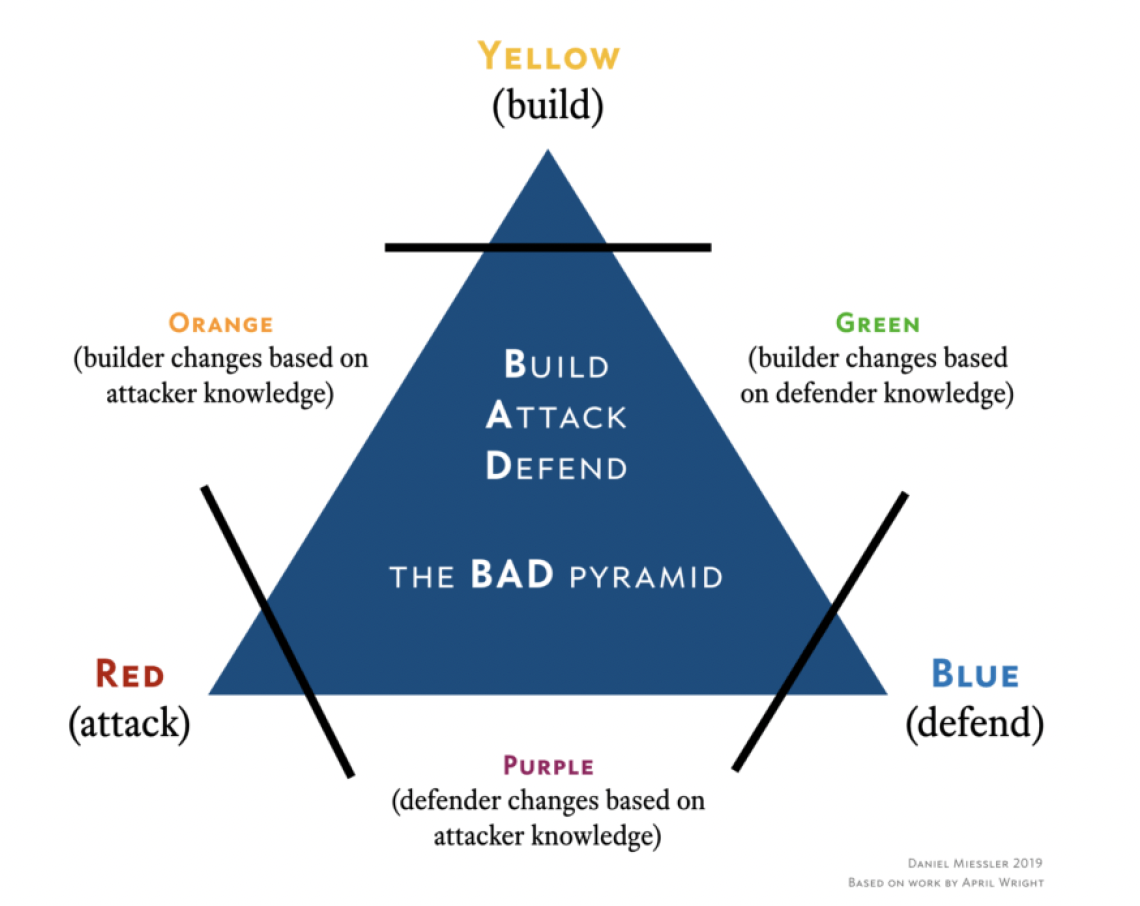
\includegraphics[width=\linewidth]{res/hacker_classification.png}
    \caption{}
\end{figure}
Gli hacker che si limitano ad eseguire e/o modificare leggermente gli exploit senza conoscerne il funzionamento prendono il nome di skid, cript kiddie, generalmente bistrattati dalla community, ma costituiscono una minaccia alla stregua dei black hat. uno skid potrebbe lanciare un script un exploit in grado di generare un Denial of Service anche come danno collaterale.

Un azienda potrebbe richiedere un'analisi del proprio livello di sicurezza delle infrastrutture o di un suo prodotto, per effettuare ciò esistono due procedure:
\begin{itemize}
    \item Vulnerability Assessment, ci si occupa di fare un analisi delle possibili vulnerabilità presenti nel sistema;
    \item Penetration Test, ci si occupa di scoprire dove un hacker, sfruttando le vulnerabilità trovate, possa arrivare.
\end{itemize}

Gli attaccanti invece seguono uno specifico processo per effettuare i propri attacchi chiamato Kill Chain.
\begin{figure}[h!]
    \centering
    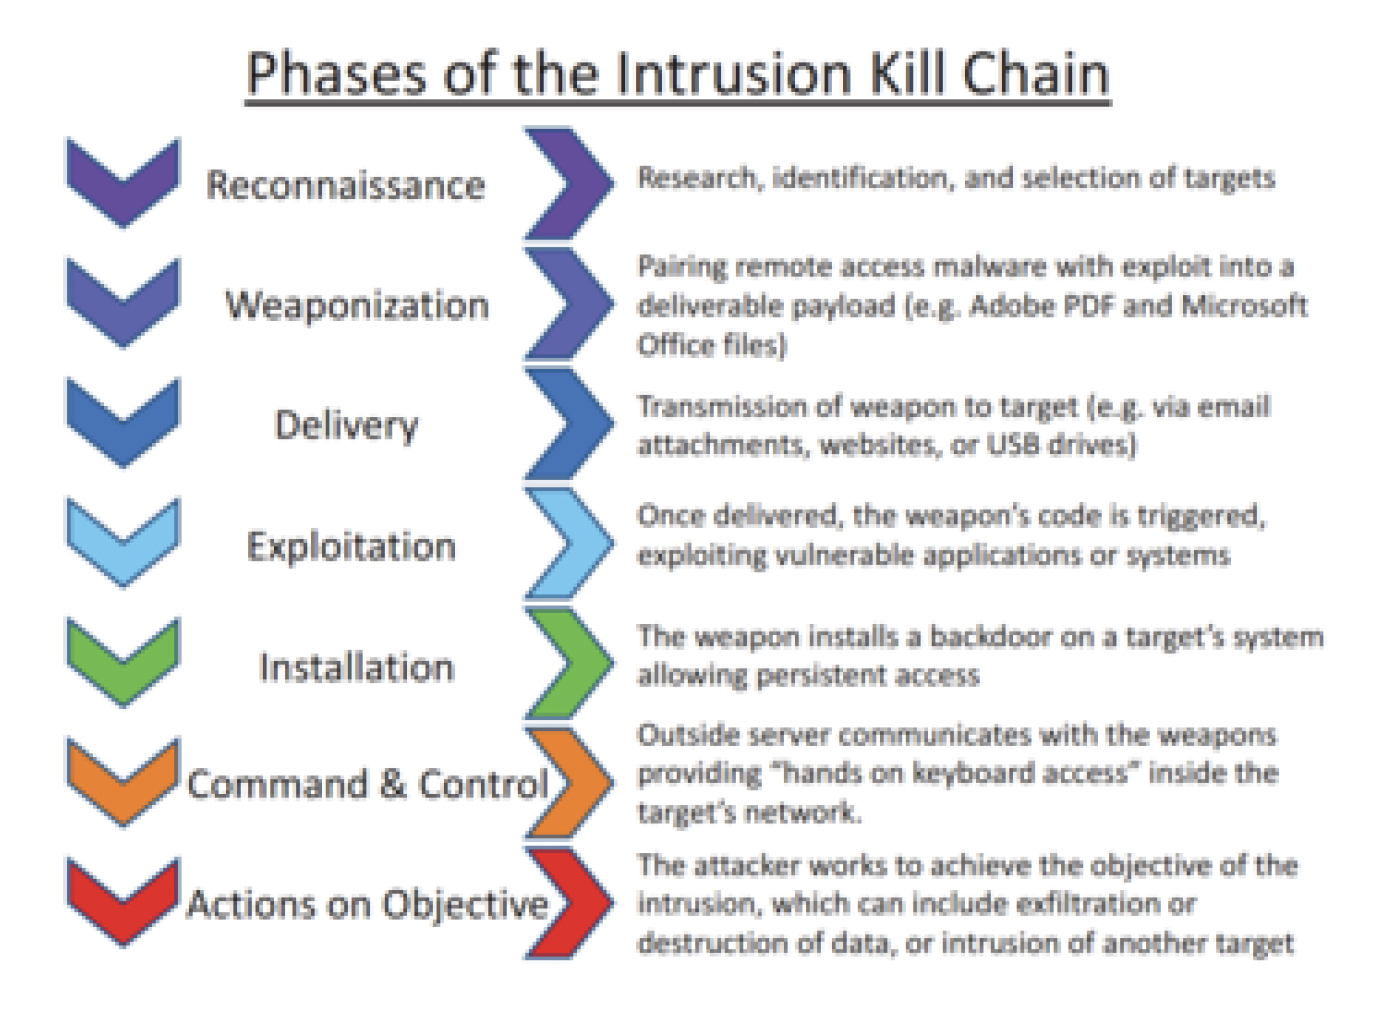
\includegraphics[width=\linewidth]{res/kill_chain.png}
    \caption{}
\end{figure}

\section{Cos'è una vulnerabilità}
In un sistema informatico una vulnerabilità è una debolezza che può essere sfruttata da una fonte terza per eseguire codice malevolo sulla macchina stessa.
\begin{figure}[h!]
    \centering
    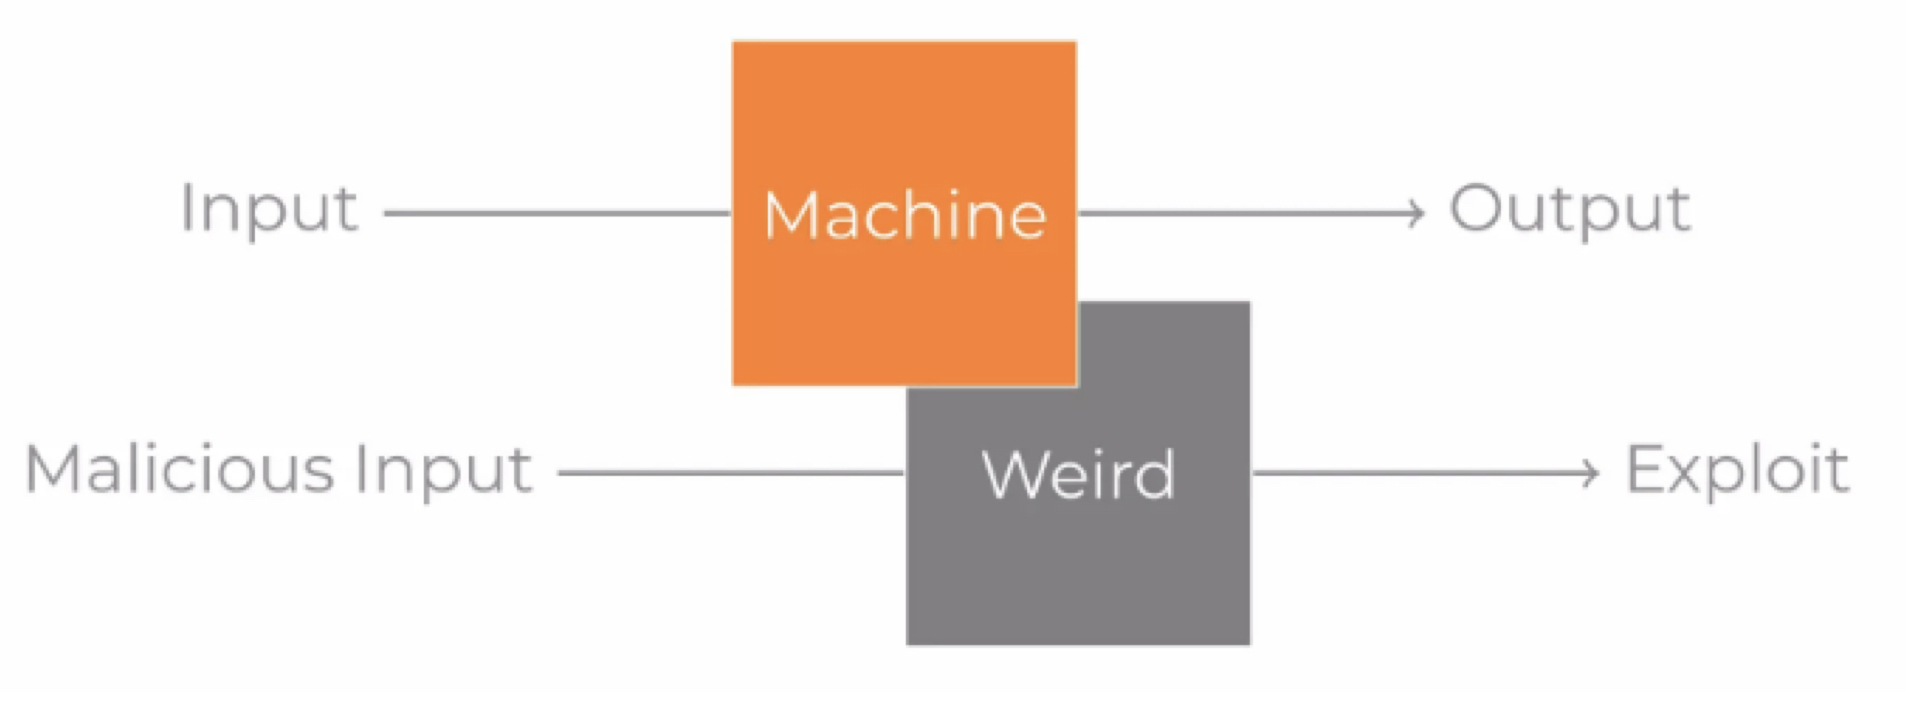
\includegraphics[width=\textwidth]{res/weird_machine.png}
    \caption{}
\end{figure}
\section{Cos'è un exploit}
In un sistema informatico un exploit è un programma, uno script o un comando in grado di sfruttare una specifica vulnerabilità per ottenere un risultato, es. Installare un malware o ottenere una shell.
Un esempio di shellshock è quanto segue:
\begin{lstlisting}[language=bash,caption={bash version}]
#!/bin/bash
curl -H "User-Agent: () {:;} /bin/eject" https://example.com
\end{lstlisting}

\section{Common Vulnerability Exposure}
Un CVE (Common Vulnerability Exposure) è un programma di classificazione delle vulnerabilità, a molte vulnerabilità note è associato un identificativo CVE con il relativo livello di minaccia.
Uno \textit{\textbf{zero day}} è una vulnerabilità precedentemente ignota a chi è interessato alla sua risoluzione.
